\chapter{Lec 04 - Informed Search II}
\section{Recursive Best First Search}
Recursive best-first search (RBFS) is a simple recursive algorithm that attempts to RECURSIVE mimic the operation of standard best-first search, but using only \textbf{linear space}.\newline\newline
Its structure is similar to that of a recursive depth-first search, but
rather than continuing indefinitely down the current path, it uses the \textit{f-limit} variable to keep track of the \textit{f-value} of the best alternative path available from any ancestor of the current node. If the current node exceeds this limit, the recursion unwinds back to the alternative path. As the recursion unwinds, RBFS replaces the \textit{f-value} of each node along the path with a \textbf{backed-up value}, that is, the best \textit{f-value} of its children. In this way, RBFS remembers the \textit{f-value} of the best leaf in the forgotten subtree and can therefore decide whether it’s worth reexpanding the subtree at some later time.
\begin{center}
    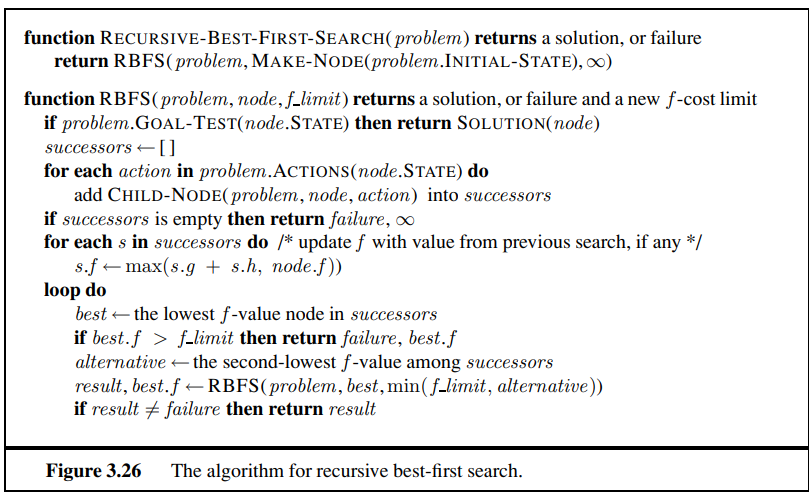
\includegraphics[scale=0.8]{images/RBFS-algo.png}
    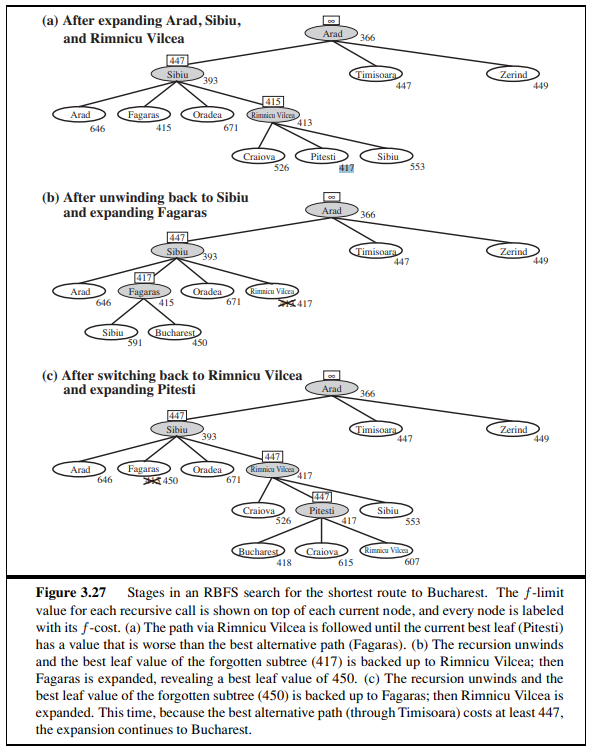
\includegraphics[]{images/RBFS.png}
\end{center}
Just like A*, RBFS is optimal if the heuristic function $h(n)$ is admissible. Moreover, it has space complexity $O(bd)$ and time complexity which is exponential in the worst case.\newline\newline
The main problem of RBFS (as well as IDA*) is the use of too little memory. In fact, it may happen that the algorithm reexpand forgotten subtrees many times to recreate the best path. Unlike A*, RBFS does not store in the frontier each expanded node, but only the nodes along a single path from the root to a leaf node. 
\newline\newline
In general, the less memory you use, more repetitions you have to do in time. The algorithm MA* (memory-bounded A*) and SMA* (simplified memory-bounded A*) \textbf{fully use all available memory}.

\section{Simplified MA*}
Simplified MA* behaves just like A*, expanding the best node until the memory is full. At this point, it cannot add a new node to the search tree without dropping an old one. SMA* always drops the worst leaf node, that is, the one with the highest \textit{f-value} (last node in the queue). Like RBFS, SMA* then backs up the value of the removed node to its parent. In this way, the ancestor of a forgotten subtree knows the quality of the best path in that subtree. With this information, SMA* regenerates the subtree only when all other paths have been shown to look worse than the path it has forgotten.\newline\newline
What if all the leaf nodes have the same \textit{f-value}? To avoid selecting the same node for deletion and expansion, SMA* expands the newest best leaf and deletes the oldest worst leaf. These coincide when there is only one leaf, but in that case, the current search tree must be a single path from root to leaf that fills all of memory. If the leaf is not a goal node, then even if it is on
an optimal solution path, that solution is \textbf{not reachable with the available memory}.\newline\newline
SMA* properties:
\begin{itemize}
    \item \textbf{complete} only if a solution can be kept in memory
    \item \textbf{optimal} only if any optimal solution is reachable (otherwise it returns the best reachable solution).
\end{itemize}

\section{Heuristic functions}
The performance of heuristic search algorithms depends on the quality of the heuristic function. Let's look, as an example, at heuristics for the 8-puzzle
\begin{center}
    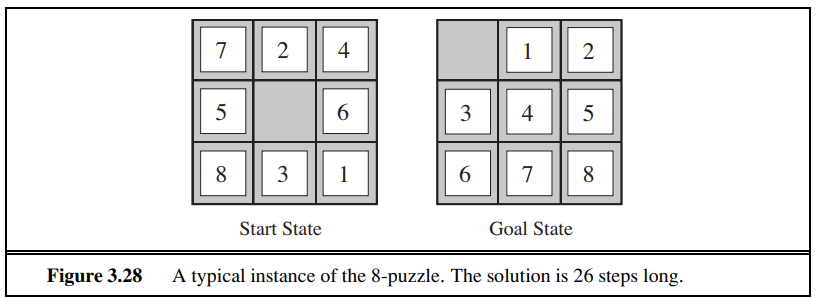
\includegraphics[]{images/8-puzzle.png}
\end{center}
If we want to find the shortest solutions by using A*, we need a heuristic function that never overestimates the number of steps to the goal. There is a long history of such heuristics for the 8-puzzle; here are two commonly used candidates:
\begin{itemize}
    \item $h_1(n) =$ number of misplaced tiles. The start state above would have $h_1(S) = 6$.
    \item $h_2(n) =$ total Manhattan distance, that is, the sum of the distances of the tiles from their goal positions. The state start $S$ qould have $h_2(S) = 4 + 0 + 3 + 3 + 1 + 0 + 2 + 1 = 14$.
\end{itemize}
$h_1$ is faster to compute than $h_2$, however, if $h_2(n) \geq h_1(n)$ for all $n$ (both admissible), then $h_2$ \textbf{dominates} $h_1$. Domination translates directly into efficiency: A* using
$h_2$ will never expand more nodes than $A*$ using $h_1$ (except possibly for some nodes with $f(n) = C^*$). Recall that $A*$ expand all nodes with $f(n) < C^*$ (which is mandatory for any optimal algorithm). This is the same as saying that every node with $h(n) < C^* - g(n)$ will surely be expanded. But because $h_2$ is at least as big as $h_1$ for all nodes, every node that is surely expanded by A* search with $h_2$ will also surely be expanded with $h_1$, and $h_1$ might cause other nodes to be expanded as well. Hence, it is generally better to use a heuristic function with higher value, provided it is consistent and that the computation time for the heuristic is not too long.\newline\newline
Admissible heuristics can be derived from the exact solution cost of
a \textbf{relaxed} version of the problem. A relaxed problem is a problem with fewer restrictions on the actions than the original.\newline\newline
If the rules of the 8-puzzle are relaxed so that a tile can move anywhere, then $h_1(n)$ gives the shortest solution. If the rules are relaxed so that a tile can cove to any adjacent square, then $h_2(n)$ gives the shortest solution.\newline\newline
The key point is that the optimal solution cost of a relaxed problem is no greater than the optimal solution cost of the real problem. Hence, the cost of an optimal solution to a relaxed problem is an \textbf{admissible} heuristic for the original problem.\newline\newline
For example, we can derive a lower bound on the shortest tour for the Travelling Salesman Problem (TSP) using a Minimum Spanning Tree (which can be computed in $O(n^2)$).

\section{Iterative Improvements Algorithms}
If the path to the goal does not matter, we might consider a different class of algorithms, ones that do not worry about paths at all. \textbf{Local search algorithms} operate using a single current node (rather than multiple paths) and generally move only to neighbors of that node. In this case, the \textbf{state space} is the set of \textit{complete} configurations and the task is to find the \textbf{optimal} configuration (e.g. TSP), or to find a configuration satisfying constraints (e.g. timetable).\newline\newline
Local search algorithms have two key advantages: (1) they use very little memory, usually a constant amount, since the paths followed by the search are not retained; and (2) they can often find reasonable solutions in large or infinite (continuous) state spaces for which systematic algorithms are unsuitable.\newline\newline
In addition to finding goals, local search algorithms are useful for solving pure optimization problems, in which the aim is to find the best state according to an \textbf{objective function}.\newline\newline
To understand local search, we find it useful to consider the state-space landscape. A landscape has both “location” (defined by the state) and “elevation” (defined by the value of the heuristic cost function or objective function). If elevation corresponds to cost, then the aim is to find the lowest valley, a \textbf{global minimum}; if elevation corresponds to an objective function, then the aim is to find the highest peak—a global maximum.  Local search algorithms explore this landscape. A complete local search algorithm always finds a goal if one exists; an optimal algorithm always finds a global minimum/maximum.
\begin{center}
    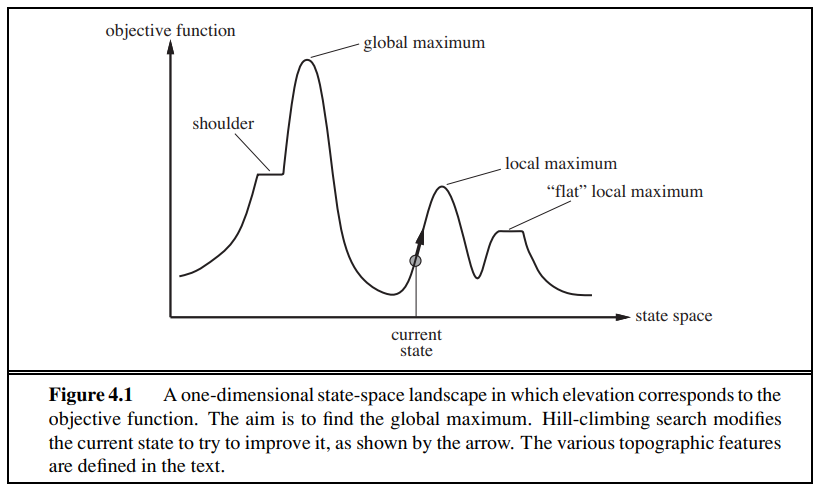
\includegraphics[scale=0.8]{images/state landscape.png}
\end{center}

\subsection{Hill-climbing}
The \textbf{hill-climbing} search algorithm is simply a loop that continually moves in the direction of increasing value, that is, uphill. At each step the current node is replaced by the best neighbor, i.e., the neighbor with the highest \textbf{value} (or lowest heuristic cost if a heuristic is used). It terminates when it reaches a “peak” where no neighbor has a higher value.
\begin{center}
    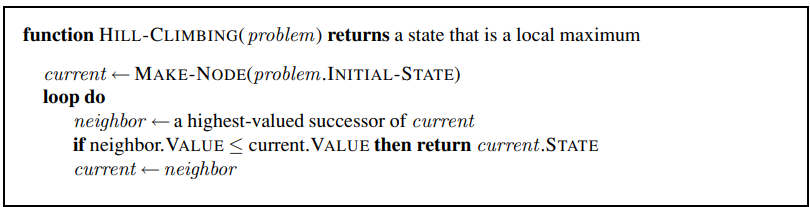
\includegraphics[]{images/hill-climbing.png}
\end{center}
To illustrate hill climbing, we will use the \textbf{8-queens problem}. Local search algorithms typically use a complete-state formulation, where each state has 8 queens on the board, one per column. The successors of a state are all possible states generated by moving a single queen to another square in the same column (so each state has $8 \times 7 = 56$ successors). The heuristic cost function $h$ is the number of pairs of queens that
are attacking each other, either directly or indirectly. The global minimum of this function is zero, which occurs only at perfect solutions.
\begin{center}
    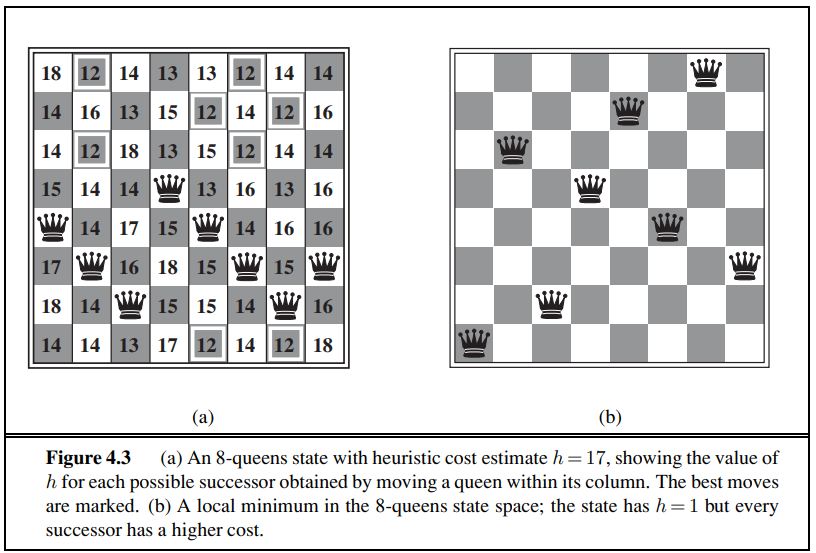
\includegraphics[scale=0.8]{images/8-queens.png}
\end{center}
Hill climbing often makes rapid progress toward a solution because it is usually quite easy to improve a bad state. Unfortunately, hill climbing often gets stuck for the following reasons:
\begin{itemize}
    \item \textbf{Local maxima:}  a local maximum is a peak that is higher than each of its neighboring states but lower than the global maximum.

    \item \textbf{Ridges:} Ridges result in a sequence of local maxima that is very difficult for greedy algorithms to navigate.

    \item \textbf{Plateaux:} a plateau is a flat area of the state-space landscape. It can be a flat local maximum, from which no uphill exit exists, or a shoulder, from which progress is possible.
\end{itemize}
A possible solution to the \textbf{plateaux} problem is to allow \textbf{sideways move}, i.e, move to a state with same $h$ value, in the hope that the plateau is really a shoulder. In fact, if we are on a flat maxima, an infinite loop will occur. The solution to above problem is to put a limit on the number of consecutive sideways moves allowed.\newline\newline
Many variants of hill climbing have been invented to face the problem of \textbf{local maxima}. \textbf{Stochastic hill climbing} chooses at
random from among the uphill moves; the probability of selection can vary with the steepness of the uphill move. This usually converges more slowly than steepest ascent, but in some state landscapes, it finds better solutions. \textbf{Random-restart hill climbing} conducts a series of hill-climbing searches from randomly generated initial states. It can be proved that if $p$ is the probability to find an optimal solution for a single
search, the expected number of searches needed to find an optimal solution is $1/p$.\newline\newline
Going back to the 8-queens problem, Starting from a randomly generated 8-queens state, \textbf{standard} steepest-ascent hill climbing gets stuck 86\% of the time, solving only 14\% of problem instances.  It works quickly, taking just 4 steps on average when it succeeds and 3 when it gets stuck, not bad for a state space with $8^8 \approx 17$ million states.\newline\newline
Hill-climbing with \textbf{sideways moves} ($\leq 100$ consecutive moves) raises the percentage of problem instances solved to 94\%. On the average it takes around 21 steps to find a solution, otherwise around 64 steps for finding suboptimal solution.\newline\newline
\textbf{Random-restart hill climbing}, for 8-queens instances with no sideways moves allowed ($p \approx 0.14$), needs roughly 7 iterations to find a goal (6 failures and 1 success). The expected number of steps is the cost of one successful iteration plus $(1-p)/p$ times the cost of failure, or roughly 22 steps in all. When we allow sideways moves, the optimal solution is found with probability $p = 0.94$ of times, thus around 1.06 searches to find optimal solution. Total expected number of steps: $63(1  p)/p + 21 = 25.08$.
